\documentclass[a4paper]{article}

\usepackage[english]{babel}
\usepackage[utf8x]{inputenc}
\usepackage[T1]{fontenc}

\usepackage[a4paper,top=3cm,bottom=3cm,left=2cm,right=2cm,marginparwidth=1.5cm]{geometry}

\usepackage{amsfonts}
\usepackage{amsmath}
\usepackage{amssymb}
\usepackage{amsthm}
\usepackage{graphicx}
\usepackage[ruled,vlined]{algorithm2e}
\usepackage[colorinlistoftodos]{todonotes}
\usepackage[colorlinks=true, allcolors=blue]{hyperref}

\setlength\parindent{0pt}

\DeclareMathOperator*{\argmax}{argmax}
\DeclareMathOperator*{\argmin}{argmin}
\newcommand*{\vertbar}{\rule[-1ex]{0.5pt}{2.5ex}}
\newcommand*{\horzbar}{\rule[.5ex]{2.5ex}{0.5pt}}

\newtheorem{theorem}{Theorem}[section]
\newtheorem{lemma}[theorem]{Lemma}

\title{CS 395T: Homework 2}
\author{Brady Zhou \\ brady.zhou@utexas.edu}

\begin{document}

\maketitle

\section{Programming}

\textbf{Problem 1.} Shape deformation (Gradient Descent) \\

We are interested in minimizing the following equation via gradient descent.
\begin{align*}
    \argmin_{p_1, \ldots, p_n, R_1, \ldots, R_n} \sum_{i=1}^n \Big( \sum_{j \in \mathcal{N}(i)} ||R_i (p_i^{rest} - p_j^{rest}) - (p_i - p_j)||^2 \Big) + \lambda \sum_{p_i \in \mathcal{H}} ||p_i - h_i||^2
\end{align*}

First, we can take the derivative with respect to $p_k$, and for notations $\gamma$ will be $1$ if $p_k \in \mathcal{H}$ and $0$ otherwise.
\begin{align*}
    &= \nabla \sum_{i=1}^n \Big( \sum_{j \in \mathcal{N}(i)} ||R_i (p_i^{rest} - p_j^{rest}) - (p_i - p_j)||^2 \Big) + \nabla \lambda \sum_{p_i \in \mathcal{H}} ||p_i - h_i||^2 \\
    &= \sum_{j \in \mathcal{N}(k)} \nabla ||R_k (p_k^{rest} - p_j) - (p_k - p_j)||^2 + \sum_{j \in \mathcal{N}(k)} \nabla ||R_j (p_j^{rest} - p_k) - (p_j - p_k)||^2 + \gamma \lambda ||p_k - h_k||^2 \\
    &= \sum_{j \in \mathcal{N}(k)}-2 (R_k (p_k^{rest} - p_j) - (p_k - p_j)) + \sum_{j \in \mathcal{N}(k)} 2 (R_j (p_j^{rest} - p_k) - (p_j - p_k)) + 2 \gamma \lambda (p_k - h_k)
\end{align*}

Next, to take the derivative with respect to $R$, we have to reparameterize $R_i$ by $c_i \in \mathbb{R}^3$. For notation, let $[c]_x$ denote the skew symmetric matrix formed by $c$. From homework 1 we can see that $R = I + \frac{1 - \cos \theta}{\theta^2} [c]_x^2 + \frac{\sin \theta}{\theta} [c]_x$, where $\theta = ||c||$. \\

For this exercise, note that $\frac{d\theta}{d c_i} = \frac{c_i}{\theta}$ first let us take $\frac{dR}{dc_x}$.
\begin{align*}
    \frac{dR}{dc_x} &= \frac{\theta^2 \sin \theta \frac{d\theta}{dc_x} - 2 (1 - \cos \theta) \theta \frac{d\theta}{d c_x}}{\theta^4} [c]_x^2 + \frac{1 - \cos \theta}{\theta^2} A_x + \frac{-\theta \cos \theta \frac{d\theta}{dc_x} - \sin \theta \theta \frac{d\theta}{dc_x}}{\theta^2} [c]_x + \frac{\sin \theta}{\theta} B_x
\end{align*}

where
\[
    A_x = \begin{bmatrix}
        0 & c_y & c_z \\
        c_y & -2 c_x & 0 \\
        c_z & 0 & -2 c_x \\
        \end{bmatrix}
    B_x = \begin{bmatrix}
        0 & 0 & 0 \\
        0 & 0 & -1 \\
        0 & 1 & 0 \\
        \end{bmatrix}
\]

Next, consider $\frac{dR}{dc_y}$.
\begin{align*}
    \frac{dR}{dc_x} &= \frac{\theta^2 \sin \theta \frac{d\theta}{dc_y} - 2 (1 - \cos \theta) \theta \frac{d\theta}{dc_y}}{\theta^4} [c]_x^2 + \frac{1 - \cos \theta}{\theta^2} A_y + \frac{-\theta \cos \theta \frac{d\theta}{dc_y} - \sin \theta \theta \frac{d\theta}{dc_y}}{\theta^2} [c]_x + \frac{\sin \theta}{\theta} B_y
\end{align*}

where
\[
    A_y = \begin{bmatrix}
        -2 c_y & c_x & 0 \\
        c_x & 0 & c_z \\
        0 & c_z & -2 c_y \\
        \end{bmatrix}
    B_y = \begin{bmatrix}
        0 & 0 & 1 \\
        0 & 0 & 0 \\
        -1 & 0 & 0 \\
        \end{bmatrix}
\]

Finally, consider $\frac{dR}{dc_z}$.
\begin{align*}
    \frac{dR}{dc_z} &= \frac{\theta^2 \sin \theta \frac{d\theta}{dc_z} - 2 (1 - \cos \theta) \theta \frac{d\theta}{dc_z}}{\theta^4} [c]_x^2 + \frac{1 - \cos \theta}{\theta^2} A_z + \frac{-\theta \cos \theta \frac{d\theta}{dc_z} - \sin \theta \theta \frac{d\theta}{dc_z}}{\theta^2} [c]_x + \frac{\sin \theta}{\theta} B_z
\end{align*}

where
\[
    A_z = \begin{bmatrix}
        -2 c_z & 0 & c_x \\
        0 & -2 c_z & c_y \\
        c_x & c_y & 0 \\
        \end{bmatrix}
    B_z = \begin{bmatrix}
        0 & -1 & 0 \\
        1 & 0 & 0 \\
        0 & 0 & 0 \\
        \end{bmatrix}
\]

Next, we must compute $\frac{df}{dR}$ for simplicity, we will now compute this element wise.
\begin{align*}
    \frac{dF}{dR_{rc}}
    &= \nabla \sum_{j \in \mathcal{H}} ||R (p^{rest} - p_j) - (p - p_j)||^2 \\
    &= \sum_{j \ in \mathcal{H}} 2 \Big( (R (p^{rest} - p_j) - (p - p_j))_r (p^{rest} - p_j)_c \Big)
\end{align*}

Now, we collect all the partials into a vector $\frac{df}{dR} \in \mathbb{R}^9$, we collect all the partials with respect to $c_i$, $\frac{dR}{dc_i} \in \mathbb{R}^9$, and do chain rule to get $\frac{df}{dc_i}$, and finally turn this into a vector $\frac{df}{dc} \in \mathbb{R}^3$.

\begin{figure}[!h]
\centering
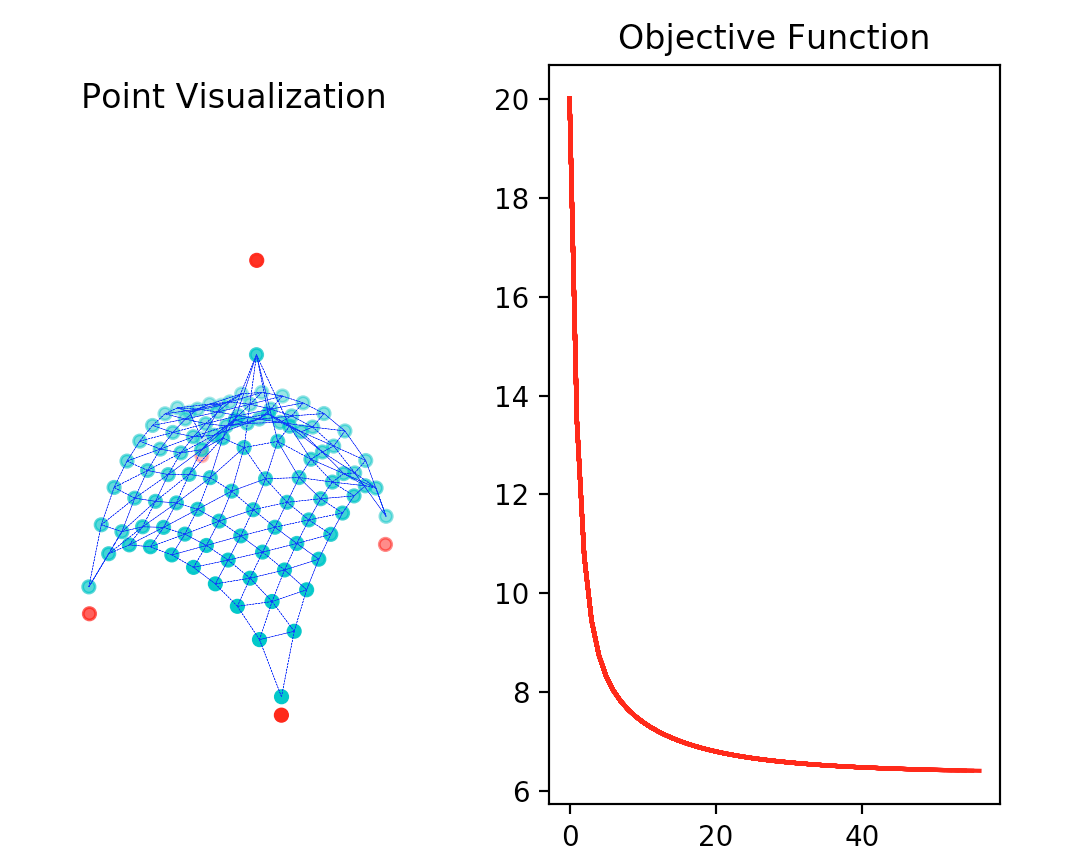
\includegraphics[width=0.3\textwidth]{cs395t_graphics_hw2_gradient1.png}
\caption{Results of gradient descent}
\end{figure}

\textbf{Problem 2.} Shape deformation (Alternating Minimization) \\

First, to calculate $p_1, \ldots, p_n$ that minimize the equation, we can write this the energy as a least squares system $Ax = b$, where $x \in \mathbb{R}^{3 n}$, is a block vector of $p_1, \ldots, p_n$,  and $A$ is a ``selector matrix'', and $b$ is a vector of block vectors of knowns. \\

To be more precise,

\[
    x = \begin{bmatrix}
        p_1 \\
        p_2 \\
        \ldots \\
        p_n \\
        \end{bmatrix}
\]

where $p_i \in \mathbb{R}^3$.

\[
    A = \begin{bmatrix}
        \horzbar A_1 \horzbar \\
        \horzbar A_2 \horzbar \\
        \ldots \\
        \horzbar A_m \horzbar \\
        \end{bmatrix}
\]

where $A_k \in \mathbb{R}^{3 \times 3n}$, and $m$ is the total number of squared norm terms. \\

Now, consider a single term in the left hand term of the energy function $R_i(p_i^{rest} - p_j^{rest}) - (p_i - p_j)$. We will decompose this into a block matrix $A_k$ and $b_k$ vector. \\

Clearly, for the known $b_k \in \mathbb{R}^3$,
\[
    b_k = \begin{bmatrix}
        \vertbar \\
        p_i^{rest} - p_j^{rest} \\
        \vertbar \\
        \end{bmatrix}
\]

Now, $A_k$ will consist of a single block $I$ for $p_i$, and a $-I$ for $p_j$.

\[
    A_k = \begin{bmatrix}
        \cdots & 1 & 0 & 0 & \cdots & -1 &  0 &  0 & \cdots \\
        \cdots & 0 & 1 & 0 & \cdots &  0 & -1 &  0 & \cdots \\
        \cdots & 0 & 0 & 1 & \cdots &  0 &  0 & -1 & \cdots \\
        \end{bmatrix}
\]

To finish the least squares formulation, consider a single of the right hand terms $\lambda ||p_i - h_i||^2$. Clearly, this is equivalent to $||\lambda^{\frac{1}{2}} p_i - \lambda^{\frac{1}{2}} h_i||^2$, which we can write in a block form.
\[
    b_k = \begin{bmatrix}
        \vertbar \\
        \lambda^{\frac{1}{2}} h_i \\
        \vertbar \\
        \end{bmatrix}
\]

\[
    A_k = \begin{bmatrix}
        \cdots & \lambda^{\frac{1}{2}} & 0 & 0 & \cdots \\
        \cdots & 0 & \lambda^{\frac{1}{2}} & 0 & \cdots \\
        \cdots & 0 & 0 & \lambda^{\frac{1}{2}} & \cdots \\
        \end{bmatrix}
\]

Now, we solve $Ax = b$ with our favorite least squares solver (note that $A$ will be sparse due to the connectivity of the mesh) and update $p_i$ with the corresponding block in $x$. \\

Next, we need to compute optimal $R_k$. This is equivalent the orthogonal Procustes problem (constrained version).
\begin{align*}
    \argmin_{R_k} \sum_{j \in \mathcal{N(k)}} ||R_k (p_k^{rest} - p_j^{rest}) - (p_k - p_j)||^2
\end{align*}

We can form two matrices $P, Q \in \mathbb{R}^{3 \times m}$, where $m = |\mathcal{N}(k)|$ such that
\[
    P = \begin{bmatrix}
        \vertbar & \  & \vertbar\\
        p_k^{rest} - p_1^{rest} & \dots & p_k^{rest} - p_m^{rest} \\
        \vertbar & \ & \vertbar\\
        \end{bmatrix}
\]

and
\[
    Q = \begin{bmatrix}
        \vertbar & \  & \vertbar\\
        p_k - p_1 & \dots & p_k - p_m \\
        \vertbar & \ & \vertbar\\
        \end{bmatrix}
\]

From this we can reformulate this into block form.
\begin{align*}
    \argmin_{R_k} \sum_{j \in \mathcal{N(k)}} ||R_k (p_k^{rest} - p_j^{rest}) - (p_k - p_j)||^2
    &= \argmin_{R_k} ||R_k P - Q||_{F} \\
    &= \argmin_{R_k} tr\Big((R_k P - Q)^\intercal (R_k P - Q)\Big) \\
    &= \argmin_{R_k} tr\Big(P^\intercal R_k^\intercal R_k P - P^\intercal R_k^\intercal Q - Q^\intercal R_k P + Q^\intercal Q \Big) \\
    &= \argmin_{R_k} tr\Big(P^\intercal P - P^\intercal R_k^\intercal Q - Q^\intercal R_k P + Q^\intercal Q \Big) \\
    &= \argmin_{R_k} tr(P^\intercal P) - tr(P^\intercal R_k^\intercal Q) - tr(Q^\intercal R_k P) + tr(Q^\intercal Q) \\
    &= \argmin_{R_k} - tr(P^\intercal R_k^\intercal Q) - tr(Q^\intercal R_k P) \\
    &= \argmin_{R_k} - 2tr(Q^\intercal R_k P) \\
    &= \argmax_{R_k} tr(Q^\intercal R_k P) \\
    &= \argmax_{R_k} tr(R_k P Q^\intercal)
\end{align*}

Now, taking the SVD of $Q P^\intercal$, let $U \Sigma V^\intercal = Q P^\intercal$.
\begin{align*}
    \argmax_{R_k} tr(R U \Sigma V^\intercal) &= \argmax_{R_k} tr(V^\intercal R U \Sigma)
\end{align*}

\begin{lemma} For $R \in SO(3)$, $\Sigma \in \mathbb{R}^{3 \times 3}$, $tr(R \Sigma)$ is maximized if $R = I$.
\end{lemma}

Let $\Sigma$ consist of column vectors $u_1, u_2, u_3$, $R$ consist of row vectors $R_1^\intercal, R_2^\intercal, R_3^\intercal$. We can see that
\begin{align*}
    tr(R \Sigma) &= R_1^\intercal u_1 + R_2^\intercal u_2 + R_3^\intercal u_3 \\
    &= ||R_1||||u_1|| cos \theta_1 + ||R_2||||u_2|| cos \theta_2 + ||R_3||||u_3|| cos \theta_3 \\
    &= \sigma_1^2 cos \theta_1 + \sigma_2^2 cos \theta_2 + \sigma_3^2 cos \theta_3
\end{align*}

Since $\sigma_i^2$ are positive, we can see this term is maximized if $R_i$ is aligned with $u_i$. Since we have that $||R_i|| = 1$ by orthogonality, and $u_i = \sigma_i b_i$, where $b_i$ is a basis vector, we can see this is maximized by $R_i = b_i$. This gives us our result that $R = I$.

\qed \\

Using the lemma, we can see that $R = V U^\intercal$ will maximize the optimization problem. However, we only have guarantees that $R \in O(3)$, not necessarily that $R \in SO(3)$. So now we have two cases. If $det(V U^\intercal) = 1$, we are done. If $det(V U^\intercal) = -1$, then we have to modify $R$ by $\hat R = V \hat \Sigma U^\intercal$, where $\hat \Sigma$ is the identity matrix $I$ with a slight modification, that $\hat \Sigma_{33} = -1$. $\hat R$ has a determinant of $1$ and is clearly orthogonal; moreover, $\hat R \in SO(3)$. \\

\begin{figure}[!h]
\centering
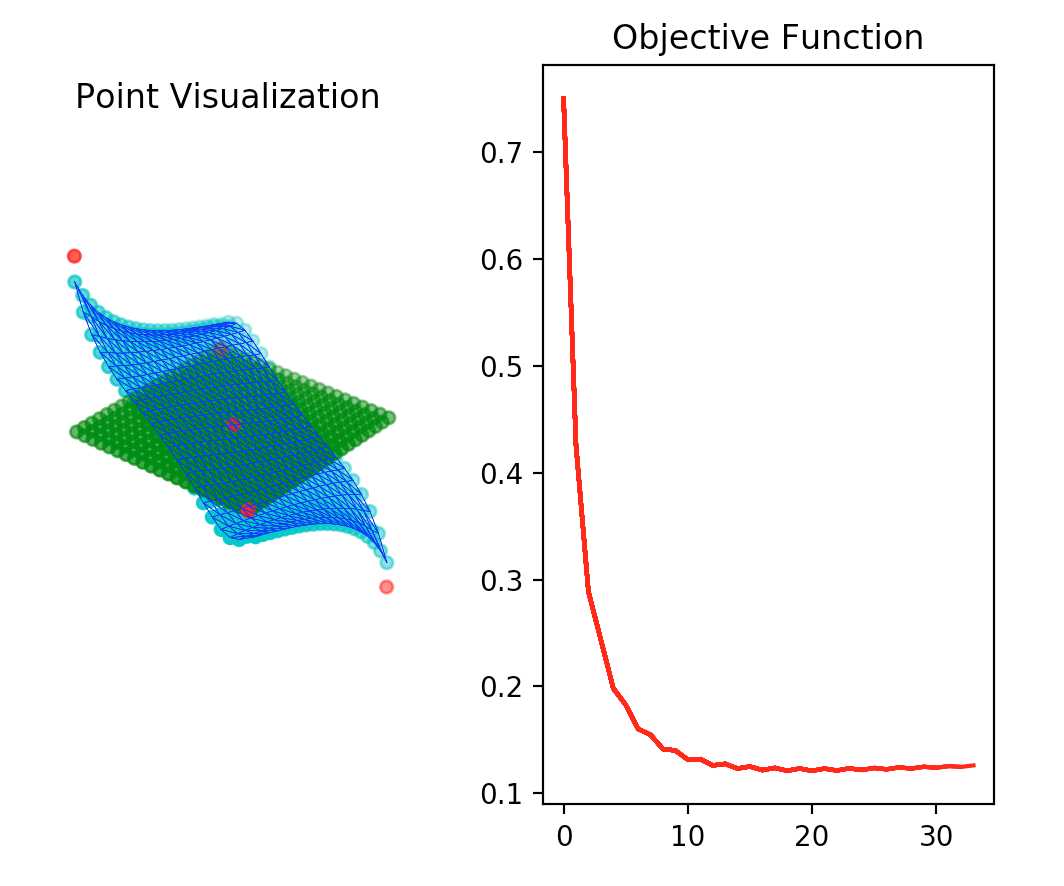
\includegraphics[width=0.3\textwidth]{cs395t_graphics_hw2_alternating.png}
\caption{Results of alternating minimization}
\end{figure}

\textbf{Problem 3a.} Finding peaks of a density (Gradient Descent) \\

This is a straightforward differentiation exercise.
\begin{align*}
    \nabla f(x) &= \nabla \Big( \sum_{i=1}^n \exp(-\frac{1}{2 \sigma^2} ||x - x_i||^2) \Big) \\
                &= \sum_{i=1}^n \exp(-\frac{1}{2 \sigma^2} ||x - x_i||^2) \Big(-\frac{1}{2 \sigma^2} \nabla (||x - x_i^2||^2) \Big) \\
                &= \sum_{i=1}^n \exp(-\frac{1}{2 \sigma^2} ||x - x_i||^2) \Big(-\frac{1}{\sigma^2} (x - x_i) \Big)
\end{align*}

Then, at every timestep, $x^{t+1} = x^t + \eta \nabla f(x^t)$, where $\eta$ is a small stepsize. \\
\begin{figure}[!h]
\centering
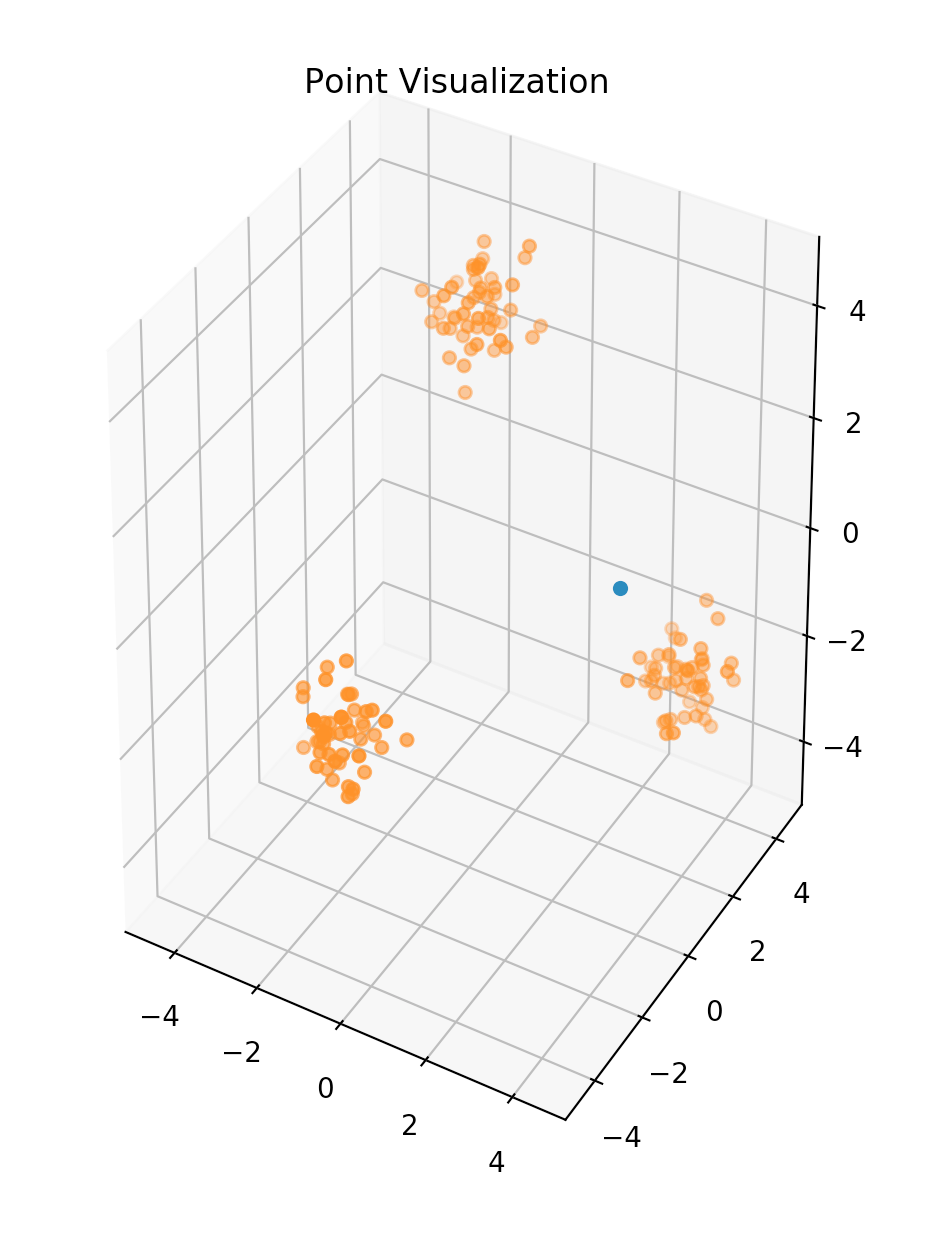
\includegraphics[width=0.3\textwidth]{cs395t_graphics_hw2_initial.png}
\caption{The unit gaussian mixtures are represented by orange points, and $x$ is represented by a single blue point. At convergence, the blue point settles in one of the clusters (intialization dependent).}
\end{figure}

\begin{figure}[!h]
\centering
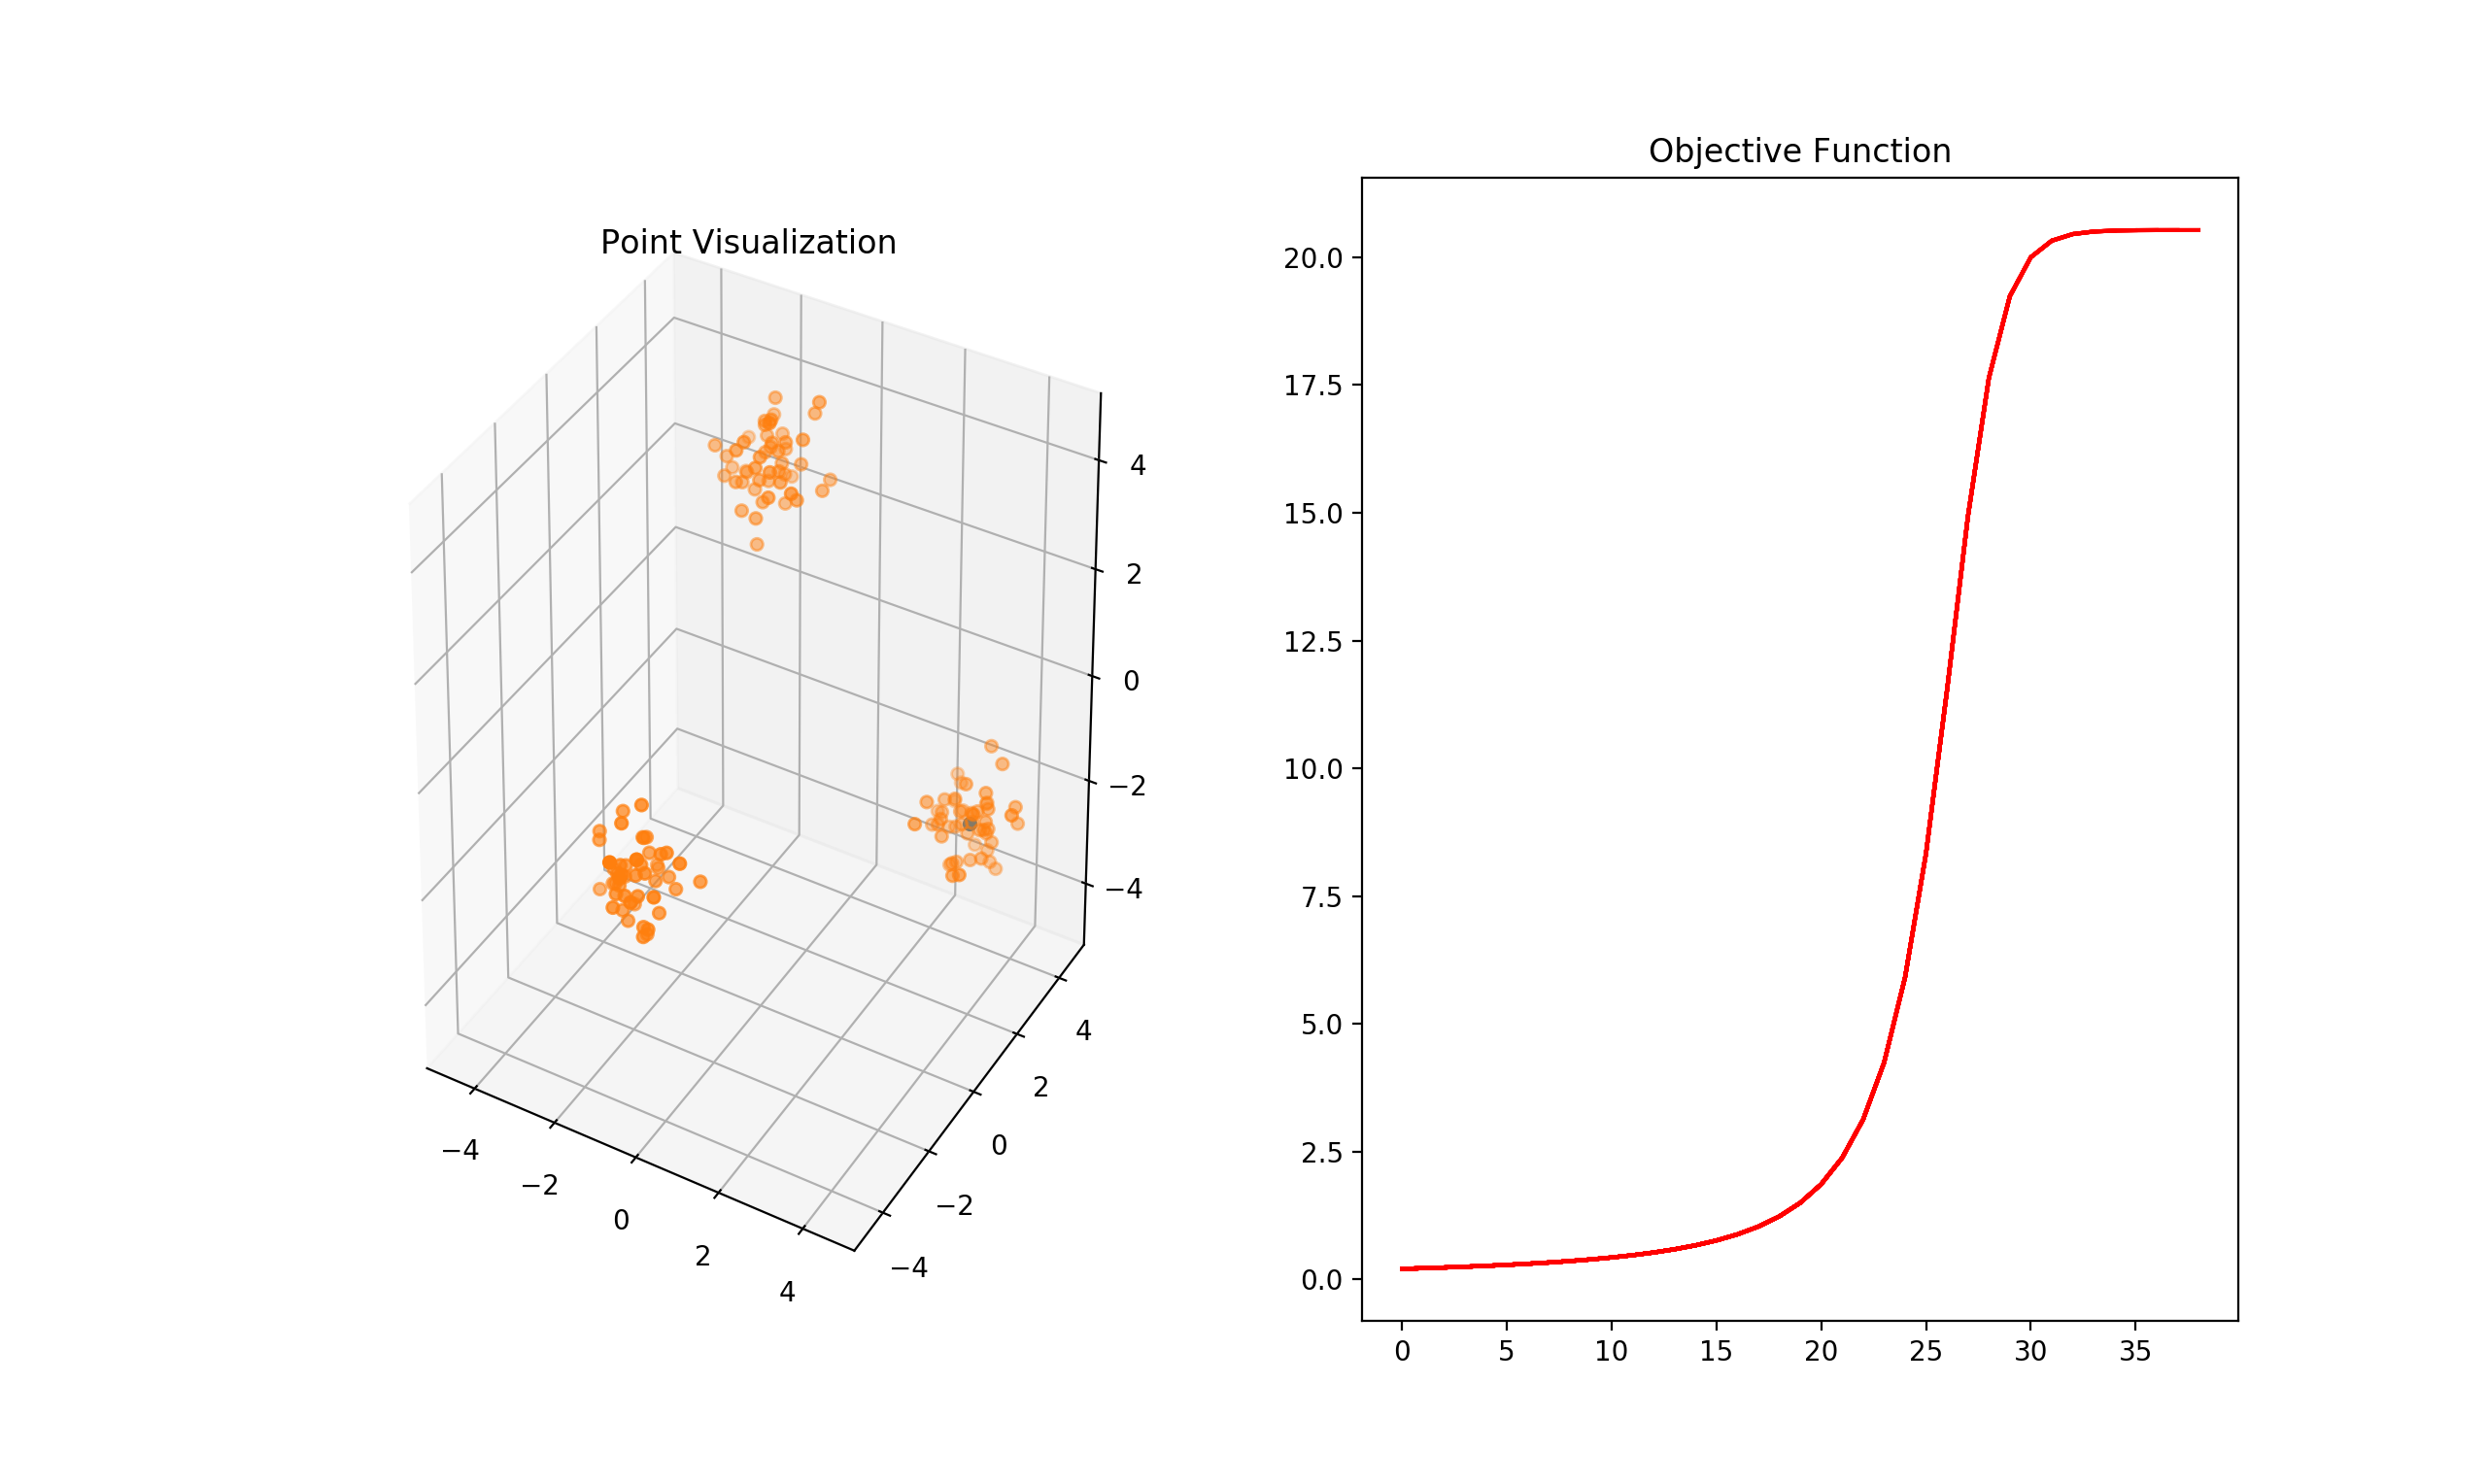
\includegraphics[width=0.5\textwidth]{cs395t_graphics_hw2_gradient.png}
\caption{Gradient ascent converges in 30 iterations.}
\end{figure}

\textbf{Problem 3b.} Finding peaks of a density (Newtons Method) \\

This is a yet another straightforward differentiation exercise.
\begin{align*}
    \nabla^2 f(x) &= \nabla \Big( \sum_{i=1}^n \exp(-\frac{1}{2 \sigma^2} ||x - x_i||^2) \Big(-\frac{1}{\sigma^2} (x - x_i) \Big) \Big) \\
                  &= \sum_{i=1}^n \exp(-\frac{1}{2 \sigma^2} ||x - x_i||^2) \Big(-\frac{1}{\sigma^2} (x - x_i) \Big) (-\frac{1}{\sigma^2} (x - x_i))^\intercal + \exp(-\frac{1}{2 \sigma^2} ||x - x_i||^2) (-\frac{1}{\sigma^2} I) \\
                  &= \sum_{i=1}^n -\frac{1}{\sigma^2} \exp(-\frac{1}{2 \sigma^2} ||x - x_i||^2) (I - \frac{1}{\sigma^2} (x - x_i) (x - x_i)^\intercal)
\end{align*}

Then, at every timestep, $x^{t+1} = x^t + \nabla^2 f(x)^{-1} \nabla f(x)$.
\begin{figure}[!h]
\centering
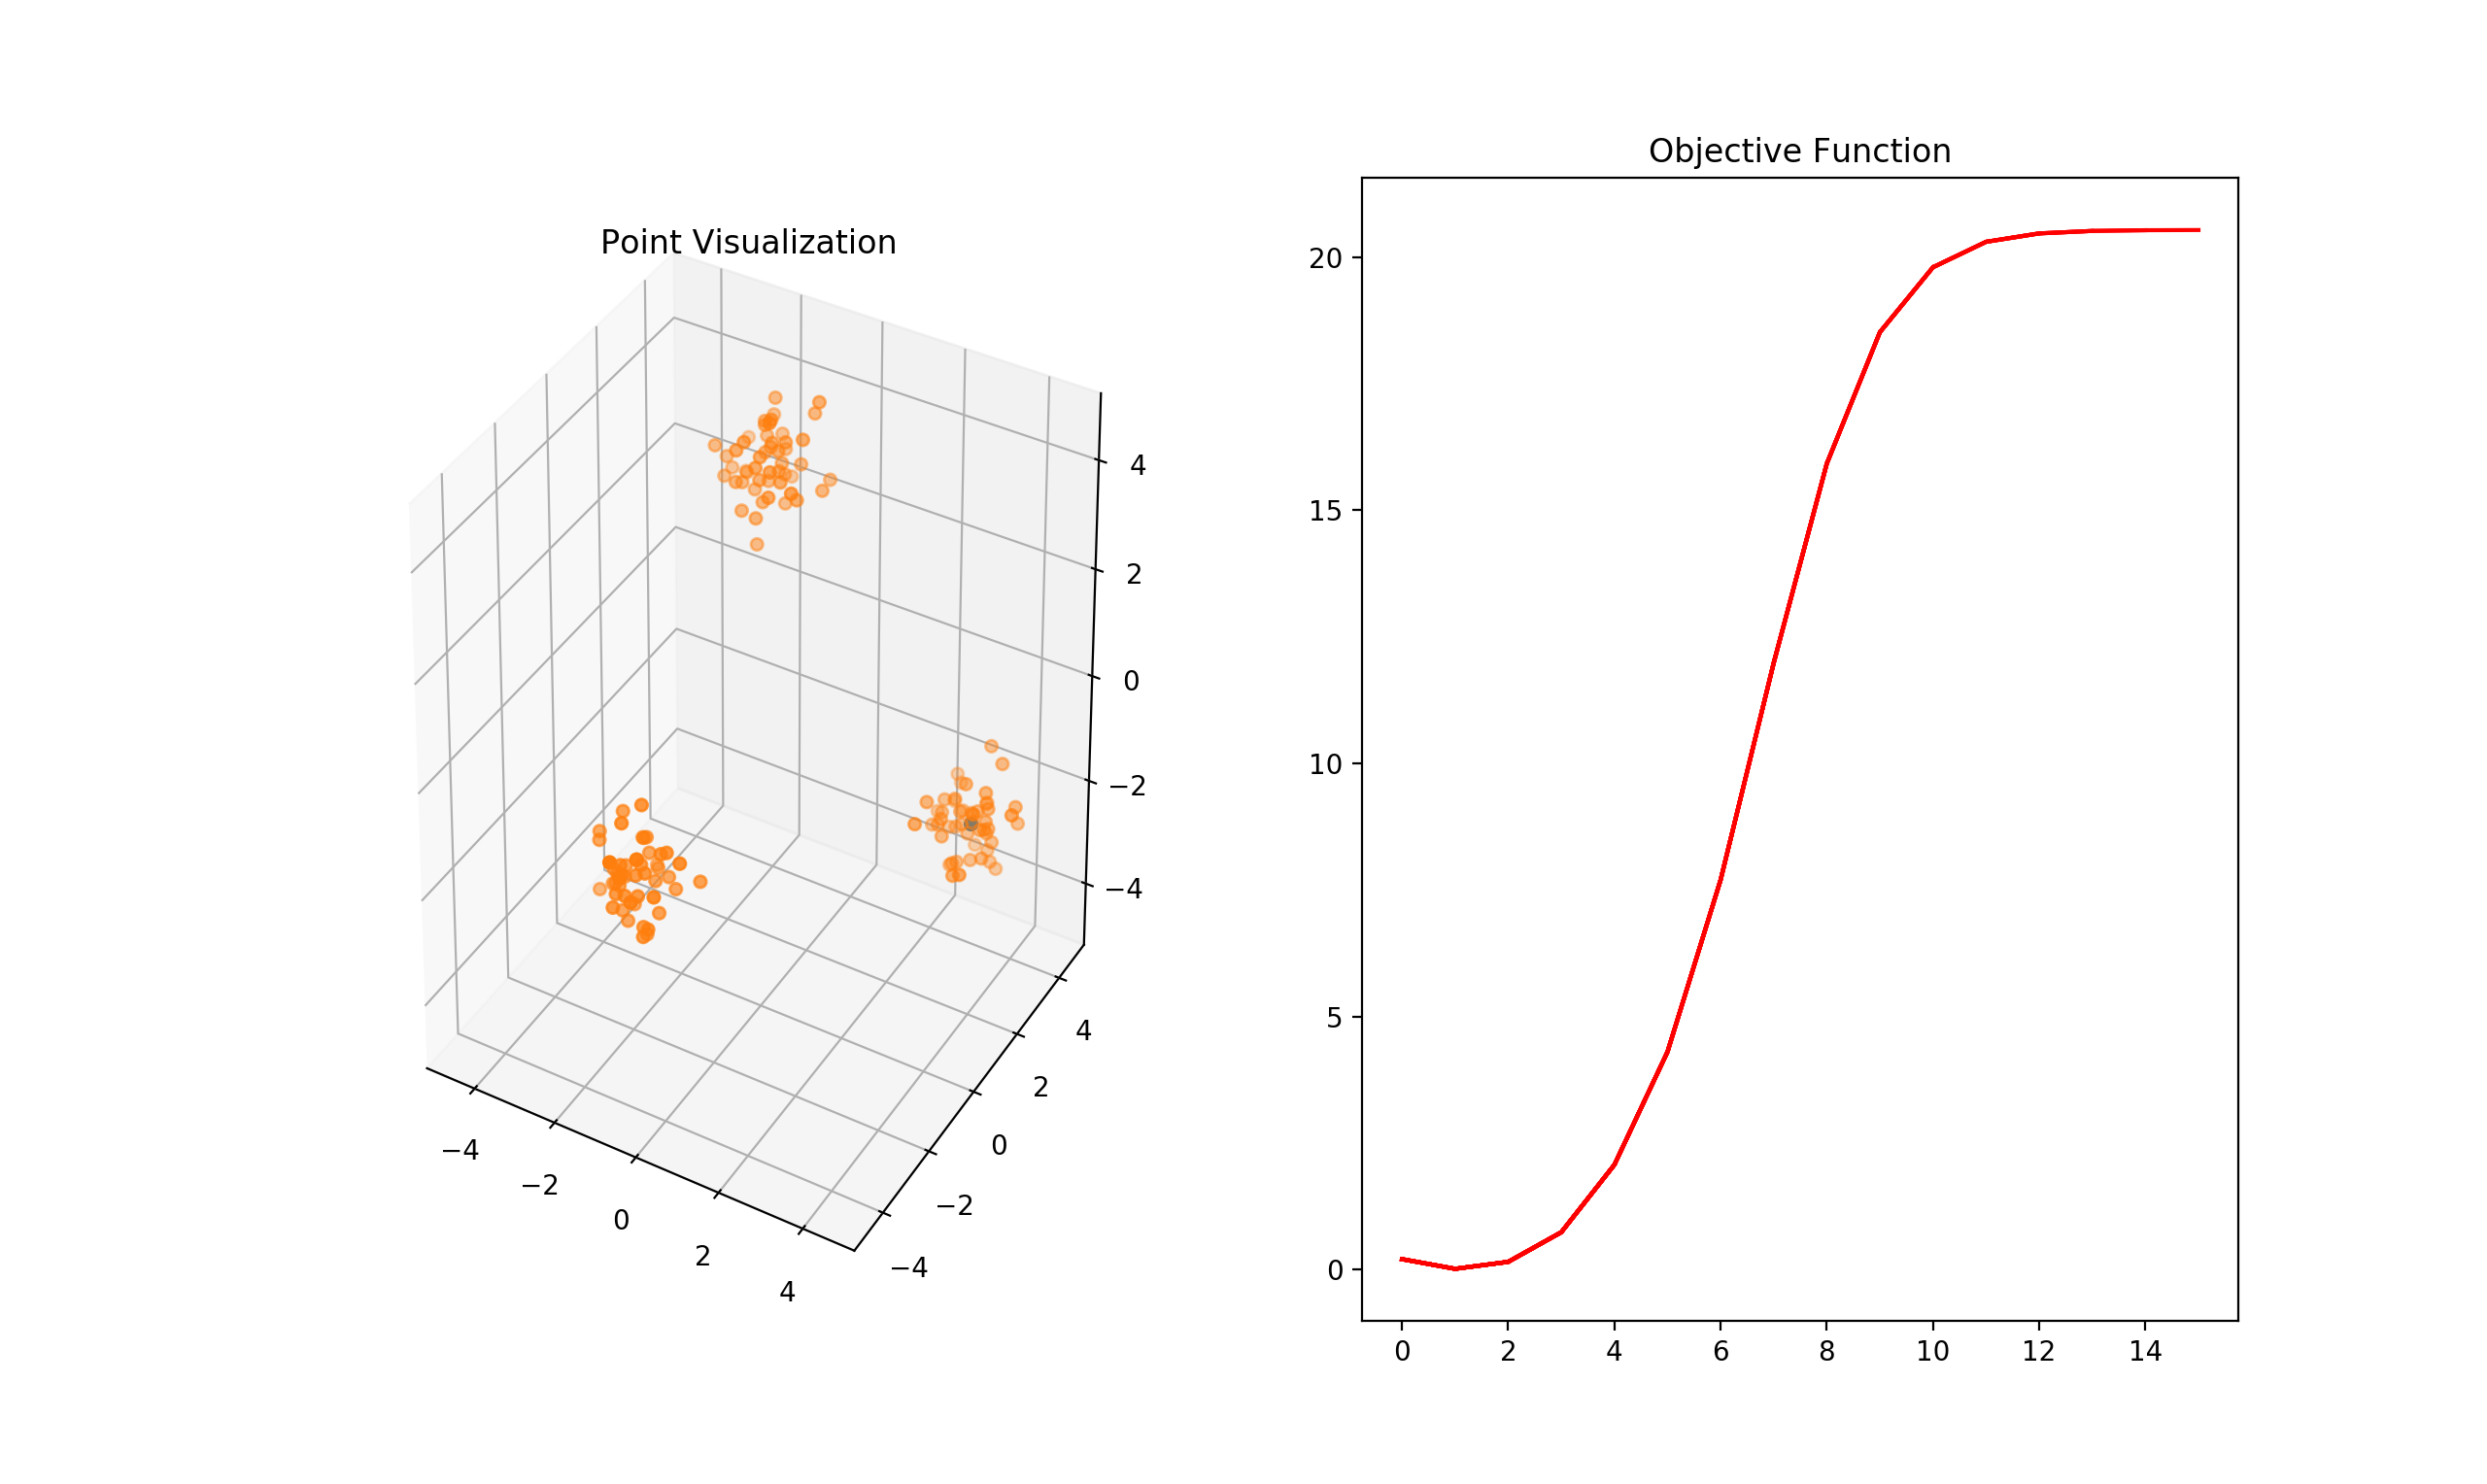
\includegraphics[width=0.5\textwidth]{cs395t_graphics_hw2_newtons.png}
\caption{Newtons Method converges in 10 iterations.}
\end{figure}

\pagebreak

\textbf{Problem 5.} If $f$ is convex and $L$-smooth, show that gradient descent with step size $\frac{1}{L}$ satisfies

\begin{align*}
    f(x_t) - f(x^*) \leq \frac{2 L ||x_o - x^*||^2}{t}
\end{align*}

First, we will need to take a side path that bounds $f(x)$ and $f(y)$ for every $x, y$ in relation to the difference of the norms. \\

\begin{lemma} $f(y) - f(x) - \nabla f(x)^\intercal (y - x) \leq \frac{L}{2} ||y - x||^2  \ \  \forall x, y$.

\begin{align*}
    f(y) - f(x) - \nabla f(x)^\intercal (y - x)
    &= \int_0^1 \frac{df}{dt} dt - \nabla f(x)^\intercal (y - x) \\
    &= \int_0^1 \nabla f(g(t))^\intercal \frac{dg}{dt} dt - \nabla f(x)^\intercal (y - x) \\
    &= \int_0^1 \nabla f(x + t (y - x))^\intercal (y - x) - \nabla f(x)^\intercal (y - x) \frac{dg}{dt} dt \\
    &= \int_0^1 \Big(\nabla f(x + t (y - x)) - \nabla f(x) \Big)^\intercal (y - x) \frac{dg}{dt} dt \\
    &\leq \int_0^1 ||\nabla f(x + t (y - x)) - \nabla f(x)||\ ||y - x|| \frac{dg}{dt} dt && \text{\normalfont By Cauchy Shwartz} \\
    &\leq \int_0^1 L ||t (y - x)||\ ||y - x|| \frac{dg}{dt} dt && \text{\normalfont By convexity} \\
    &= \int_0^1 L t ||y - x||^2 \frac{dg}{dt} dt \\
    &= \frac{L}{2} ||y - x||^2
\end{align*}

\qed
\end{lemma}

Using this lemma, we can bound the gap $f(x_{t+1}) - f(x_t)$.
\begin{align*}
    f(x_{t+1}) - f(x_t) &\leq \nabla f(x_t)^\intercal (x_{t+1} - x_t) + \frac{L}{2} ||x_{t+1} - x_t||^2 && \text{By lemma} \\
                        &= \nabla f(x_t)^\intercal (- \frac{1}{L} \nabla f(x_t)) + \frac{L}{2} ||x_{t+1} - x_t||^2 \\
    &= -\frac{1}{L} ||\nabla f(x_t)||^2 + \frac{1}{2L} ||\nabla f(x_t)||^2 \\
    &= -\frac{1}{2L} ||\nabla f(x_t)||^2 && (\star)
\end{align*}

With a bit more algebraic manipulation -
\begin{align*}
    f(x_{t+1}) &\leq f(x_t) - \frac{1}{2L} ||\nabla f(x_t)||^2 \\
               &\leq f(x^*) + \nabla f(x_t)^\intercal (x_t - x^*) - \frac{1}{2L} ||\nabla f(x_t)||^2 && \text{By convexity}
\end{align*}

To simplifify this term we need another algebraic trick.
\begin{align*}
    ||x_{t+1} - x^*||^2
    &= ||x_t - \frac{1}{L} \nabla f(x_t) - x^*||^2 && \text{By gradient step} \\
    &= ||-\frac{1}{L} \nabla f(x_t) + (x_t - x^*)||^2  \\
    &= \frac{1}{L^2} ||\nabla f(x_t)||^2 - \frac{2}{L} \nabla f(x_t)^\intercal (x_t - x^*) + ||x_t - x^*||^2
\end{align*}

So clearly,
\begin{align*}
    -\frac{L}{2} \Big( ||x_{t+1} - x^*||^2 - ||x_t - x^*||^2 \Big)
    &= -\frac{1}{2L} ||\nabla f(x_t)||^2 + \nabla f(x_t)^\intercal (x_t - x^*) && (\star \star)
\end{align*}

With this, we have that
\begin{align*}
    f(x_{t+1})
    &\leq f(x^*) + \nabla f(x_t)^\intercal (x_t - x^*) - \frac{1}{2L} ||\nabla f(x_t)||^2 \\
    &= f(x^*) - \frac{L}{2} \Big( ||x_{t+1} - x^*||^2 - ||x_t - x^*||^2 \Big) && \text{By } (\star \star)
\end{align*}

From this, we have a closed form for $\sum_{i=1}^t f(x_i) \leq t f(x^*) - \frac{L}{2} ||x_t - x^*||^2 + \frac{L}{2} ||x_0 - x^*||^2$ as all the alternating terms cancel out. \\

Finally, we are ready to show the initial claim.
\begin{align*}
    f(x_t) - f(x^*)
    &\leq \frac{1}{t} \sum_{i=1}^t (f(x_i) - f(x^*)) && \text{Since the gap is decreasing} \\
    &\leq -\frac{L}{2t} ||x_t - x^*||^2 + \frac{L}{2t} ||x_0 - x^*||^2 && \text{From above sum with algebra} \\
    &\leq \frac{L}{2t} ||x_0 - x^*||^2 && \text{Since the left term is negative} \\
    &\leq \frac{2L}{t} ||x_0 - x^*||^2
\end{align*}

\qed

\end{document}
